\documentclass[12pt,a4paper,twocolumn]{article}
\usepackage[utf8]{inputenc}
\usepackage[T1]{fontenc}
\usepackage{polski}
\usepackage[polish]{babel}
\usepackage{geometry}
\geometry{margin=2.5cm}
\usepackage{graphicx}
\usepackage{tabularx}
\usepackage{booktabs} 
\usepackage{hyperref}
\usepackage{bookmark}
\usepackage{enumitem}
\usepackage{titlesec}
\usepackage{microtype}
\usepackage{varwidth}
\usepackage{float}
\usepackage{stfloats}
\usepackage{caption}
\title{
    \begin{center}
    
\includegraphics[width=\textwidth]{../data/fig/logo.png}
    \vspace{0.25cm}
    \end{center}
    \textbf{\huge Projektowanie i analiza algorytmów} \\
    \vspace{0.5cm}
    \textit{Porównanie efektywności algorytmów sortowania przez scalanie, quicksort i kubełkowego na rzeczywistym zbiorze danych}
    }
\author{Piotr Frąc}
\date{Kwiecień 2026}


\begin{document}
\maketitle

\section{Wprowadzenie}
Niniejszy projekt dotyczy analizy efektywności trzech algorytmów 
sortowania: sortowania przez scalanie (merge sort), sortowania szybkiego (quicksort) 
oraz sortowania kubełkowego (bucket sort). 
\subsubsection*{Sortowanie przez scalanie (Merge Sort)}
Merge sort jest algorytmem opartym na paradygmacie „dziel i zwyciężaj". 
Tablica wejściowa jest rekurencyjnie dzielona na dwie równe połowy aż do uzyskania
tablic jednoelementowych, które są z definicji posortowane. Następnie podtablice 
są scalane parami w sposób zachowujący porządek elementów.
\begin{table}[H]
\centering
\begin{tabular}{ll}
Przypadek     & Złożoność  \\ \hline
Pesymistyczny & O(n log n) \\ \hline
Średni        & O(n log n) \\ \hline
Optymistyczny & O(n log n) \\ \hline
\end{tabular}
\end{table}

\subsubsection*{Sortowanie szybkie (Quicksort)}
Quicksort również wykorzystuje paradygmat „dziel i zwyciężaj". 
Wybierany jest element osiowy (pivot), względem którego tablica jest dzielona
na dwie części: elementy mniejsze od pivota i elementy większe lub równe. 
Proces jest następnie rekurencyjnie powtarzany dla obu podtablic. W implementacji użyto 
pivota jako elementu środkowego tablicy, co zmniejsza ryzyko wystąpienia 
przypadku pesymistycznego.

\begin{table}[H]
\centering
\begin{tabular}{ll}
Przypadek     & Złożoność  \\ \hline
Pesymistyczny & O($n^2$) \\ \hline
Średni        & O(n log n) \\ \hline
Optymistyczny & O(n log n) \\ \hline
\end{tabular}
\end{table}

\subsubsection*{Sortowanie kubełkowe (Bucket Sort)}
Bucket sort jest algorytmem nieporównawczym, co oznacza że nie opiera się 
na wzajemnym porównywaniu elementów. Zamiast tego wykorzystuje znajomość zakresu 
wartości danych. Elementy są rozdzielane do kubełków odpowiadających poszczególnym wartościom, 
a następnie kubełki są składane w posortowaną sekwencję.

\begin{table}[H]
\centering
\begin{tabular}{ll}
Przypadek     & Złożoność  \\ \hline
Pesymistyczny & O(n + k) \\ \hline
Średni        & O(n + k) \\ \hline
Optymistyczny & O(n + k) \\ \hline
\end{tabular}
\end{table}

\section{Meotdyka badań}
Eksperymenty przeprowadzono na zbiorze danych IMDb 
zawierającym oceny filmów w postaci liczb całkowitych z 
zakresu 0–10. Dane wczytano z pliku CSV, pomijając wpisy z pustym
polem oceny. Łącznie załadowano 962 903 rekordów.

\subsubsection*{Struktury danych}
Każdy rekord reprezentowany był przez obiekt klasy 
MovieRating zawierający identyfikator filmu, tytuł 
oraz ocenę (pole rating typu całkowitego).

\subsubsection*{Procedura pomiarowa}
Dla każdego algorytmu i każdego rozmiaru danych wykonano 
10 powtórzeń pomiaru. Przed każdym pomiarem dane były 
kopiowane z oryginalnej tablicy do tablicy pomocniczej, co 
gwarantowało że każdy algorytm operował na identycznych, 
nieposortowanych danych wejściowych.
Czas sortowania mierzony był za pomocą std::chrono::steady\_clock z 
rozdzielczością nanosekund — wyłącznie dla operacji sortowania, 
bez uwzględnienia czasu kopiowania danych ani obliczania statystyk.

\newpage
\subsubsection*{Zestawy danych}
Testy przeprowadzono dla czterech rozmiarów danych:
\begin{table}[H]
\centering
\begin{tabular}{ll}
Rozmiar & Opis \\ \hline
10 000 & Mały zestaw \\ \hline
100 000 & Średni zestaw \\ \hline
500 000 & Duży zestaw \\ \hline
962 903 & Maksymalny rozmiar \\ \hline
\end{tabular}
\end{table}

\subsubsection*{Mierzone wielkości}
Dla każdego pomiaru rejestrowano:  
\begin{itemize}
    \item Czas sortowania w nanosekundach
    \item Średnią arytmetyczną ocen (avg)
    \item Dominantę (modę) ocen (mean) 
\end{itemize}

Weryfikacja poprawności zaimplementowanych algorytmów przeprowadzana była 
automatycznie po każdym wykonaniu sortowania. 
Wykorzystano w tym celu funkcję standardowej biblioteki 
C++ std::is\_sorted, która sprawdza czy elementy tablicy 
są ułożone w porządku niemalejącym:


\subsubsection*{Stanowisko badawcze}
Eksperymenty przeprowadzono na komputerze wyposażonym w procesor 
Intel Core i5-620 (architektura 64-bitowa) oraz 8~GB pamięci RAM DDR3 
taktowanej z częstotliwością 1600~MT/s. System operacyjny to 
Kali GNU/Linux 2026.1. Kod źródłowy skompilowano kompilatorem 
g++ w wersji 15.2.0-15.

\section{Wyniki}
Poniższa tabela przedstawia uśrednione czasy sortowania z 10~powtórzeń
dla każdego algorytmu i rozmiaru danych.

\twocolumn[{%
\begin{@twocolumnfalse}
    \centering
    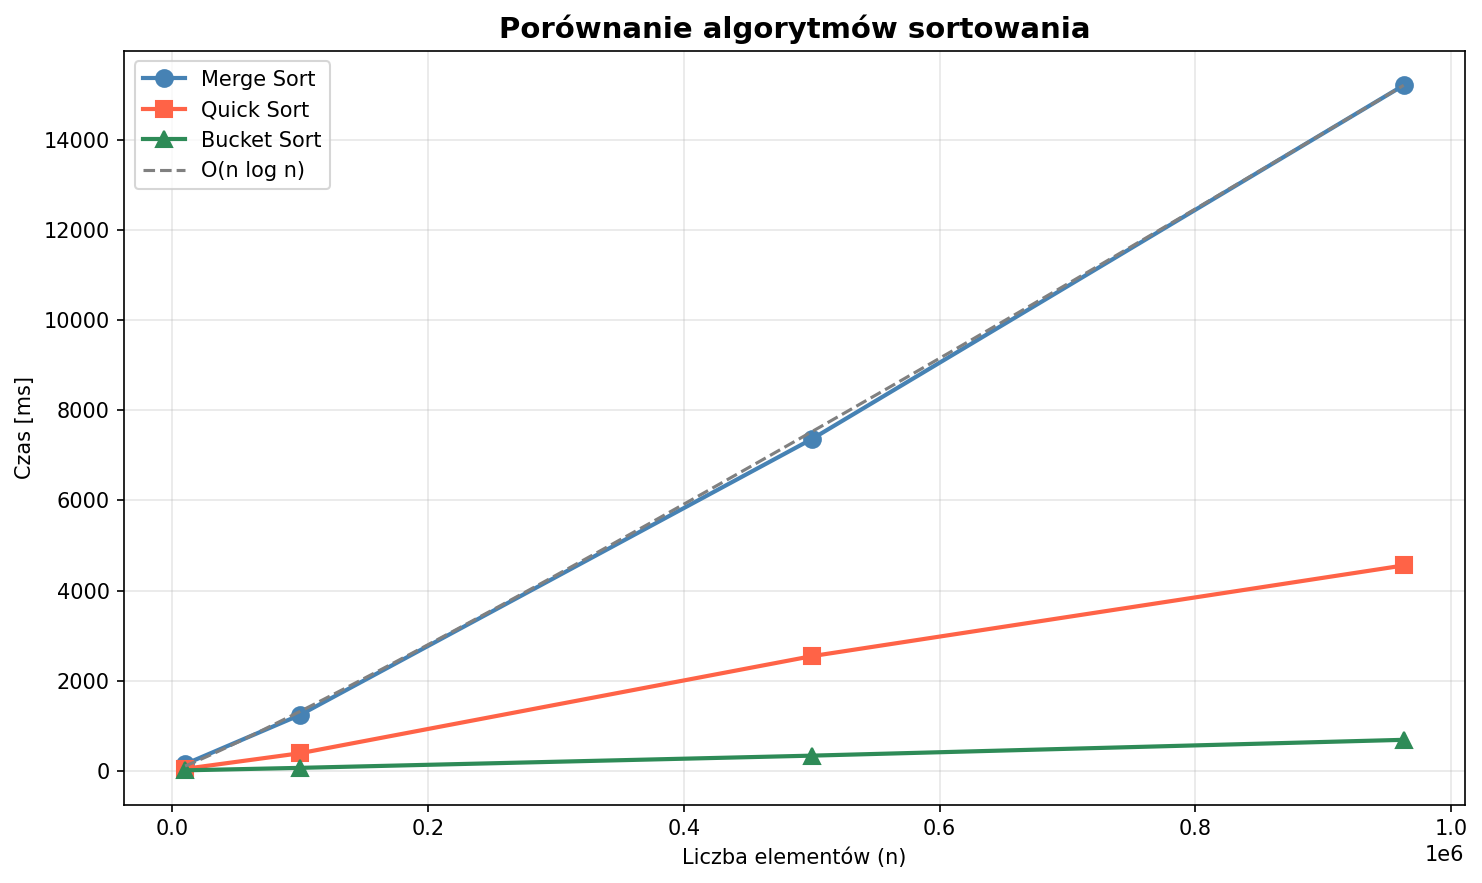
\includegraphics[width=0.8\textwidth]{../data/fig/porownanie_sortowania.png}
    \captionof{figure}{Porównanie czasu sortowania algorytmów}
    \label{fig:porownanie}
    \vspace{1em}
\end{@twocolumnfalse}
}]
\vspace{4em}
\begin{table}[H]
\centering
\footnotesize
\begin{tabular}{rrrr}
\toprule
 n & Bucket sort & Quick sort & Merge sort \\
    & {[ms]}      & {[ms]}     & {[ms]}     \\
\midrule
10~000  & 11,06   & 44,90     & 148,30    \\
100~000 & 65,95   & 390,65    & 1~241,02  \\
500~000 & 336,76  & 2~543,44  & 7~358,58  \\
962~903 & 687,84  & 4~556,43  & 15~209,67 \\
\bottomrule
\end{tabular}
\caption{Uśrednione czasy sortowania algorytmów}
\end{table}


Statystyki zbioru danych były identyczne niezależnie od zastosowanego
algorytmu, co potwierdza poprawność wszystkich implementacji.

\begin{table}[H]
\centering
\begin{tabular}{rrr}
\toprule
$n$ & Średnia ocen & Dominanta \\
\midrule
10~000  & 5,46 & 1  \\
100~000 & 6,09 & 10 \\
500~000 & 6,67 & 10 \\
962~903 & 6,64 & 10 \\
\bottomrule
\end{tabular}
\caption{Statystyki zbioru danych IMDb}
\end{table}

\section{Wnioski}
Przeprowadzone eksperymenty ujawniły wyraźne różnice w efektywności
badanych algorytmów na analizowanym zbiorze danych.

Najszybszym algorytmem okazał się \textbf{bucket sort}, który dla
962~903 elementów osiągnął czas 687,84~ms. Wynik ten potwierdza
teoretyczną złożoność liniową O($n + k$), gdzie $k = 11$ odpowiada
liczbie możliwych wartości ocen (0--10). Dzięki temu bucket sort
wykonuje jedynie trzy liniowe przejścia przez dane: zliczanie
wystąpień, wypełnianie kubełków i składanie wyniku --- bez żadnych
porównań między elementami. Jest to algorytm szczególnie efektywny
gdy zakres wartości $k$ jest mały względem liczby elementów $n$,
co w tym przypadku jest spełnione.

\textbf{Quick sort} zajął drugie miejsce z czasem 4~556,43~ms dla
pełnego zbioru danych, czyli około 6,6-krotność czasu bucket sorta.
Pomimo teoretycznej złożoności O($n \log n$), na danych z zaledwie
11 unikalnymi wartościami quicksort wykonuje wiele zbędnych porównań
i przestawień elementów o identycznych wartościach. Warto jednak
zauważyć że krzywa czasowa quicksorta jest zbliżona do
O($n \log n$), co potwierdza wykres.

\textbf{Merge sort} okazał się najwolniejszym algorytmem ---
dla 962~903 elementów osiągnął czas 15~209,67~ms, czyli ponad
22-krotność czasu bucket sorta i ponad 3-krotność czasu quicksorta.
Mimo gwarantowanej złożoności O($n \log n$), merge sort ponosi
znaczny narzut wynikający z konieczności alokacji pomocniczej
tablicy przy każdym scalaniu oraz dużej liczby operacji kopiowania
danych w pamięci.

\end{document}